\section{Implementación}
Se realiza la implementación del acoplador sobre un PCB. La inductancia es fabricada según las especificaciones desarrolladas anteriormente.

\begin{figure}[H]
    \centering
    \includegraphics[width=0.5\linewidth]{fig/pcb.png}
    \caption{acoplador montado en PCB}
    \label{fig:enter-label}
\end{figure}

\subsection{Respuesta en Frecuencia}
Para medir $f_0$ sobre el circuito implementado, se debe de realizar una medición indirecta. Esto se debe a que el instrumental (generador de onda, osciloscopio, cables, etc) introduce una capacidad en paralelo con el circuito, modificando el valor de $C$. También se debe medir con una resistencia en serie que limite la corriente que entrega el generador, puesto que el circuito en resonancia tiene una resistencia muy baja, que puede ocasionar la destrucción del mismo.

\begin{figure}[H]
    \centering
    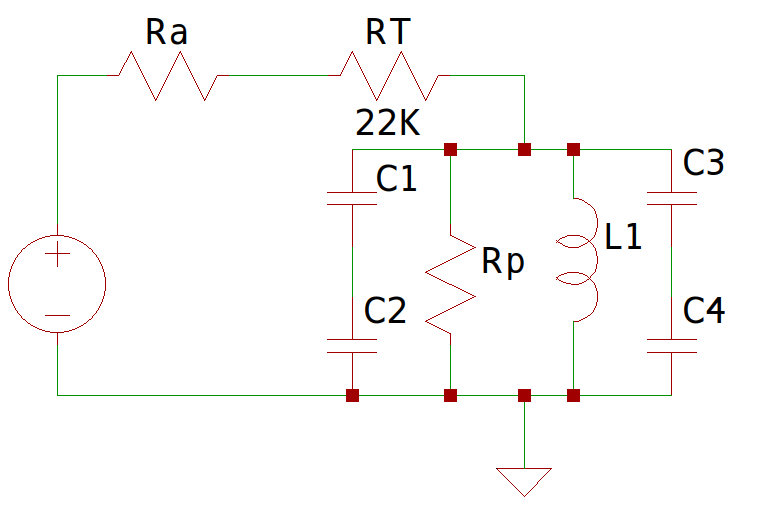
\includegraphics[width=0.5\linewidth]{fig/esqm.png}
    \caption{esquema de medición del circuito}
    \label{fig:enter-label}
\end{figure}

La resistencia $R_T$ se encuentra en el orden de la resistencia de pérdida $R_P$.

A partir de medir la caída de tensión en el acoplador, se encuentra que la frecuencia de resonancia $f'_0$ 

\begin{figure}[H]
    \centering
    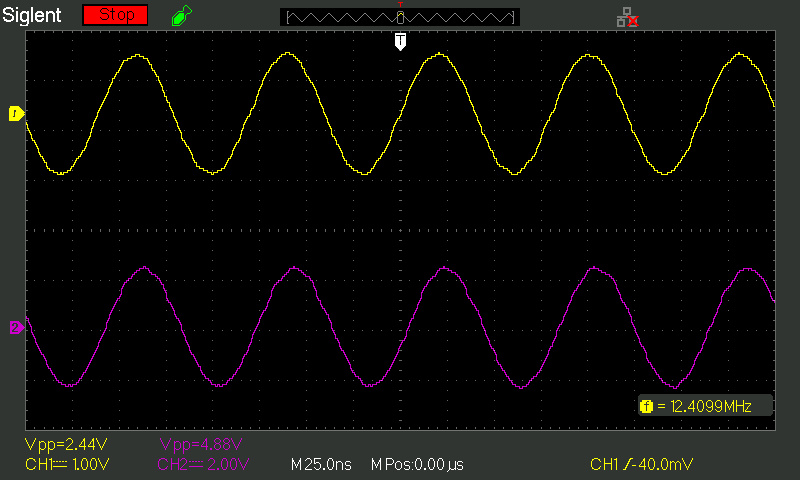
\includegraphics[width=0.5\linewidth]{oscilo/SDS00003.jpg}
    \caption{caída de tensión en el acoplador en $f'_0$}
    \label{fig:enter-label}
\end{figure}
$$
f'_0 = 12.5MHz
$$

Como la capacidad $C_X$ agregada por el instrumental es indefinida, realizamos una segunda medición, agregando en paralelo con el osciloscopio una capacidad $C_F$ de $68pF$.

\begin{figure}[H]
    \centering
    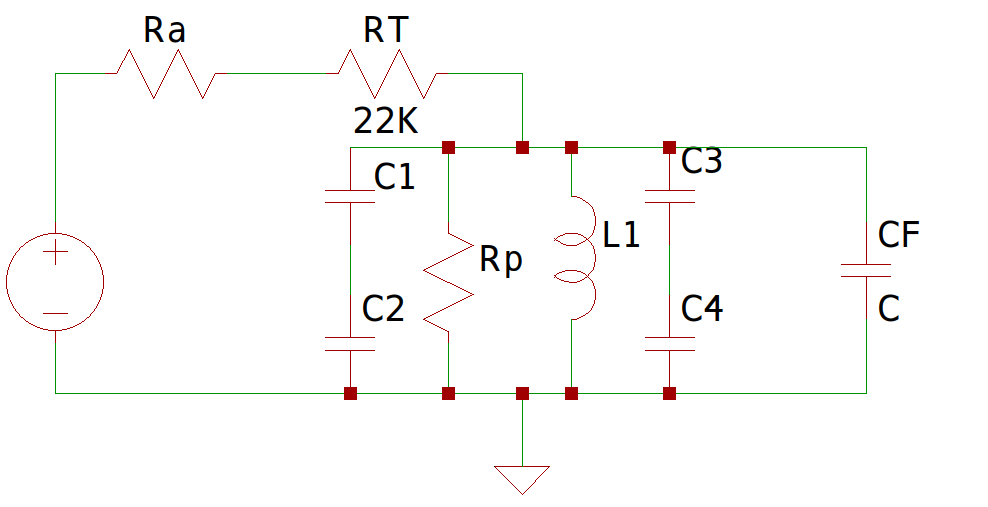
\includegraphics[width=0.5\linewidth]{fig/ctest.png}
    \caption{se agrega una capacidad conocida $C_F$}
    \label{fig:enter-label}
\end{figure}

Se mide la frecuencia de resonancia $f''_o$.

\begin{figure}[H]
    \centering
    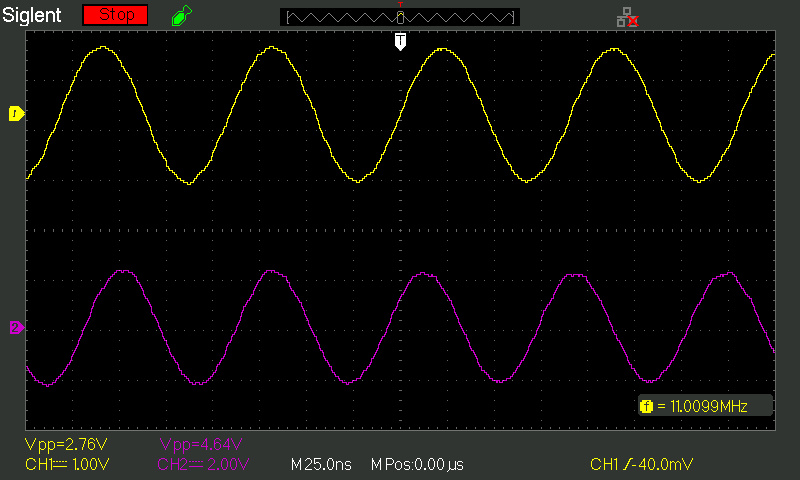
\includegraphics[width=0.5\linewidth]{oscilo/SDS00004.jpg}
    \caption{caída de tensión en el acoplador en $f''_0$}
    \label{fig:enter-label}
\end{figure}

$$
f'_0 = 11.0MHz
$$

Finalmente, se procede a calcular la capacidad inducida por el instrumental $C_X$.

$$
f'_0 = \frac{1}{2\pi\sqrt{L(C+C_X}}
$$

$$
f''_0 = \frac{1}{2\pi\sqrt{L(C+C_X+C}}
$$

Realizando el cociente entre $f'_{0}$ y $f''_{0}$ y elevando al cuadrado ambos términos se obtiene

$$
{\frac{f'_{0}}{f''_{0}}^2} = \frac{C+C_X+C_F}{C+C_X}
$$

Reordenando y reemplazando los valores obtenidos

$$
C_X = \frac{C({f''_{0}}^2-{f'_{0}}^2)+C_F*{f''_{0}}^2}{{f'_{0}}^2-{f''_{0}}^2} = 129.46pF
$$

De este valor, se puede despejar el valor del inductor

$$
L = {\frac{1}{2\pi*f'_0}}^2*1/(C+C_X) = 511nHy
$$

Por lo tanto, la frecuencia de corte del circuito medido es

$$
f_0 = \frac{1}{2\pi\sqrt{LC}} = 18.18 MHz
$$

\section{Impedancia de Entrada y Salida}

De forma análoga a la realizada en la simulación, la impedancia de entrada está dada por la diferencia entre la caída de tensión en la entrada del circuito con y sin el acoplador conectado.

\begin{figure}[H]
    \centering
    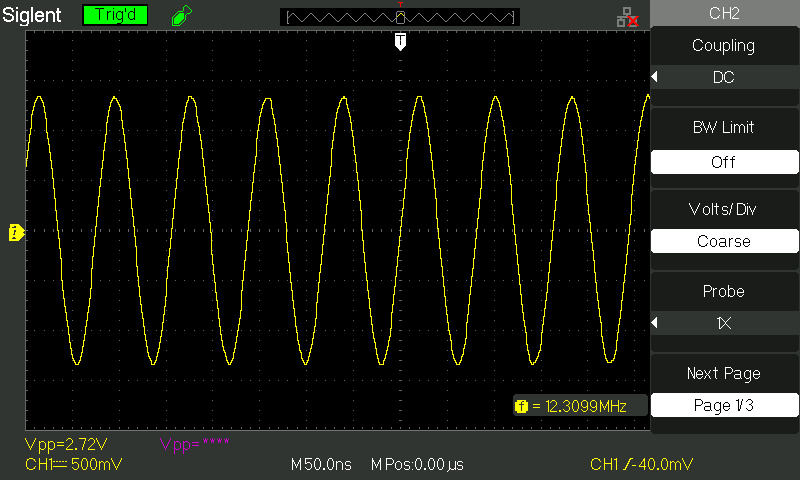
\includegraphics[width=0.5\linewidth]{oscilo/SDS00010.jpg}
    \caption{salida del generador}
    \label{fig:enter-label}
\end{figure}

\begin{figure}[H]
    \centering
    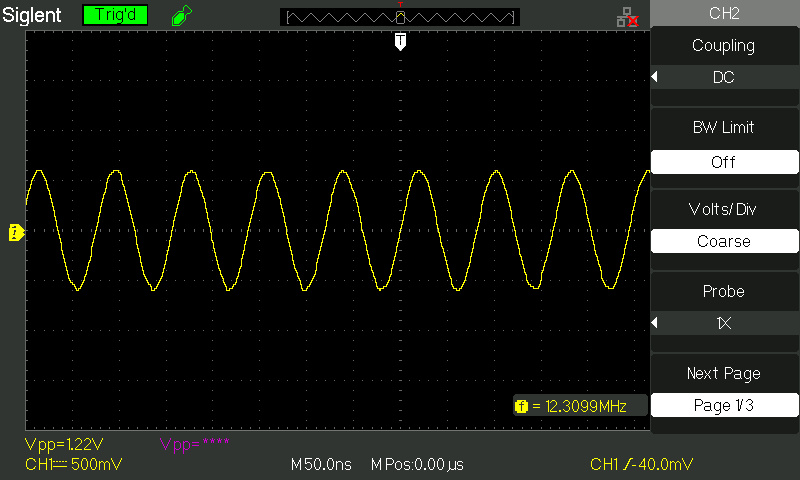
\includegraphics[width=0.5\linewidth]{oscilo/SDS00011.jpg}
    \caption{medición de la impedancia de entrada}
    \label{fig:enter-label}
\end{figure}

Se observa que la tensión en la entrada cae a aproximadamente la mitad al conectar el acoplador para la frecuencia de resonancia, lo cual indica una impedancia correctamente adaptada. Matemáticamente, esto es

$$
Z_{in} = \frac{R_a}{Vg/Vi-1} = \frac{50\Omega}{2.72V/1.16-1} = 40.66\Omega
$$

La impedancia de salida se puede medir al contrastar la caída de tensión sobre la salida del acoplador al conectar y desconectar la carga.

\begin{figure}[H]
    \centering
    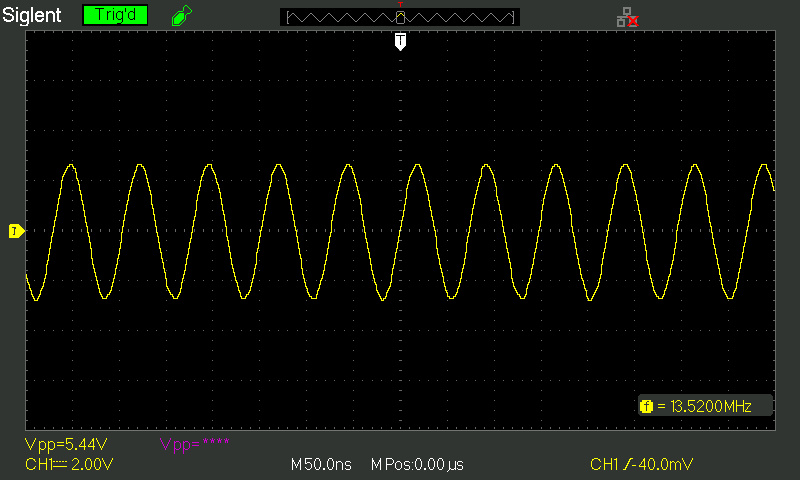
\includegraphics[width=0.5\linewidth]{oscilo/SDS00018.jpg}
    \caption{medición de la tensión de salida con carga}
    \label{fig:enter-label}
\end{figure}

\begin{figure}[H]
    \centering
    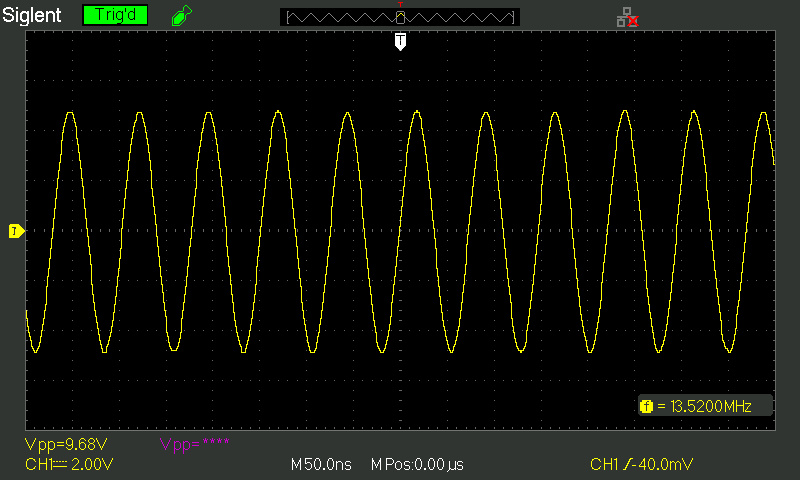
\includegraphics[width=0.5\linewidth]{oscilo/SDS00017.jpg}
    \caption{medición de la tensión de salida sin carga}
    \label{fig:enter-label}
\end{figure}


$$
Z_{out} = R_L(\frac{V_O}{V_L}-1)= 1K\Omega(\frac{9.68V}{5.44V}-1)=0.77K\Omega
$$

\subsection{Ancho de Banda}
A partir de los 3db de atenuación en la carga del acoplador, se tiene

\begin{figure}[H]
    \centering
    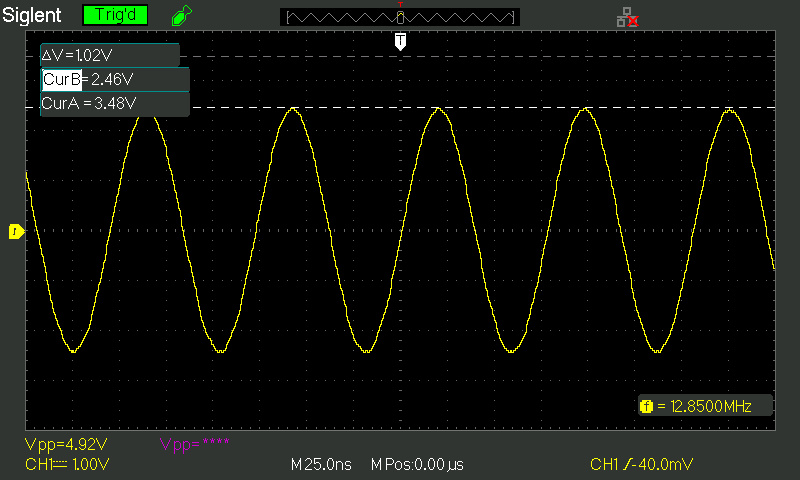
\includegraphics[width=0.5\linewidth]{oscilo/SDS00021.jpg}
    \caption{límite inferior de ancho de banda}
    \label{fig:enter-label}
\end{figure}

\begin{figure}[H]
    \centering
    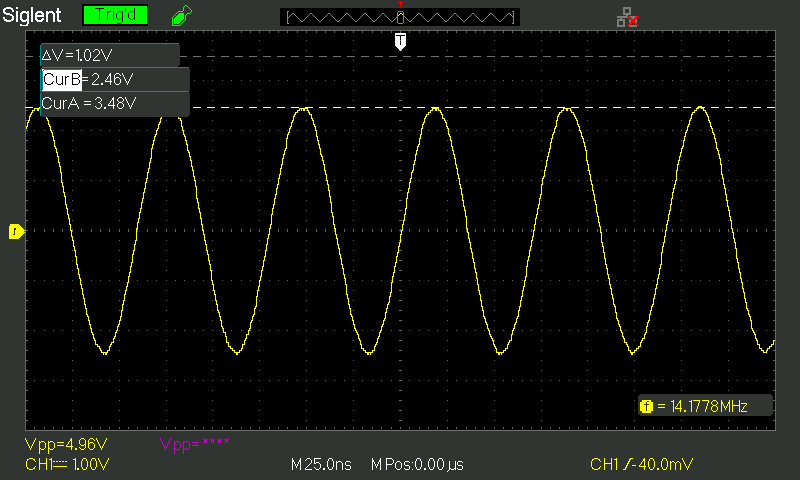
\includegraphics[width=0.5\linewidth]{oscilo/SDS00022.jpg}
    \caption{límite superior de ancho de banda}
    \label{fig:enter-label}
\end{figure}


$$
BW = 14.17MHz - 12.85MHz = 1.32MHz
$$


\subsection{Resistencia de Pérdida del Inductor, Qc y Qd}

A partir de la medición de $f'0$, en resonancia poseemos un divisor resistivo conformado por $R_a$, $R_T$ y $R_P$.

\begin{figure}
    \centering
    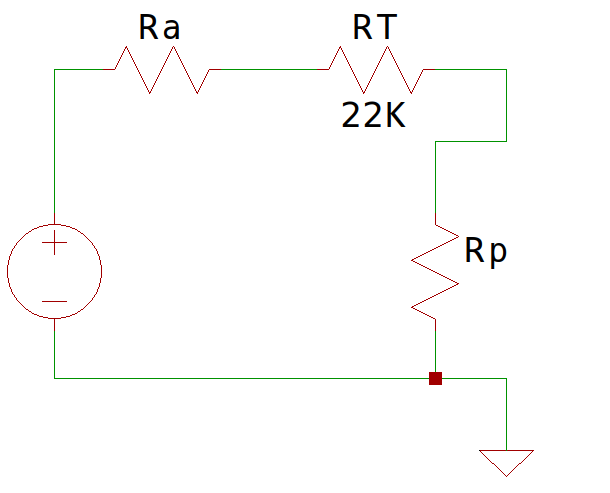
\includegraphics[width=0.5\linewidth]{fig/rp.png}
    \caption{esquema para la medición de $R_p$}
    \label{fig:enter-label}
\end{figure}

Entonces

$$
R_P = \frac{R_a+R_T}{V_i/V_o-1} = 22K\Omega
$$

A su vez, de los parámetros obtenidos podemos calcular

$$
Q_c = \frac{f_o}{BW} = 13.71
$$
$$
Q_d = \frac{R_P}{2\pi L} = 379,30 
$$


